\pagebreak[4]
\section{More Optional Rules}
\par

\textbf{Historical Reinforcements}

Instead of constructing legions as desired, the Roman player receives reinforcements on a more or less historical schedule.

The Romans have up to six additional legions that will enter the game as reinforcements during the course of the game. The legions that can enter are marked on the turn track. The exact turn they enter depends on the turn and, in most cases, a die roll during the Roman Reinforcement Phase.

Beginning on turn 1 (58 BC) the XIII and XIV legions are eligible to enter the game. On turn 1 they enter on a roll of 1-2. Roll a die for each legion individually. On turn 2 they enter on a roll of 1-3. On turn 4 they both enter automatically if they have not already entered.

Beginning on turn 5 (54 BC) both the I and XV legions are eligible to enter the game. Roll a die for each unit individually. On turn 5 they enter on a roll of 1-3. On turn 6 they enter on a 1-4. On turn 7 they enter automatically if they have not already entered.

Legions V and VI enter the game at the end of any turn in which the Massive Revolt event is played, and Vercingetorix was brought into play.

\textit{Designer's Note: Historically Caesar finished the campaign with 11 legions. He originally started with four legions - VII, VIII, IX and X - but recruited two more legions before launching his campaign, legions XI and XII (Book 1, Chapter 24). The following winter he recruited two more legions - XIII and XIV (Book 2, Chapter 2). Pompey loaned Legion I to Caesar after legion XIV was destroyed. Legions V and VI were recruited in response to Vercingetorix in 52 BC.}

\textbf{Restricted Naval Movement}

Only Roman units and Barbarian units with a naval symbol may use naval movement. Other units may not invade, move or retreat via naval move.

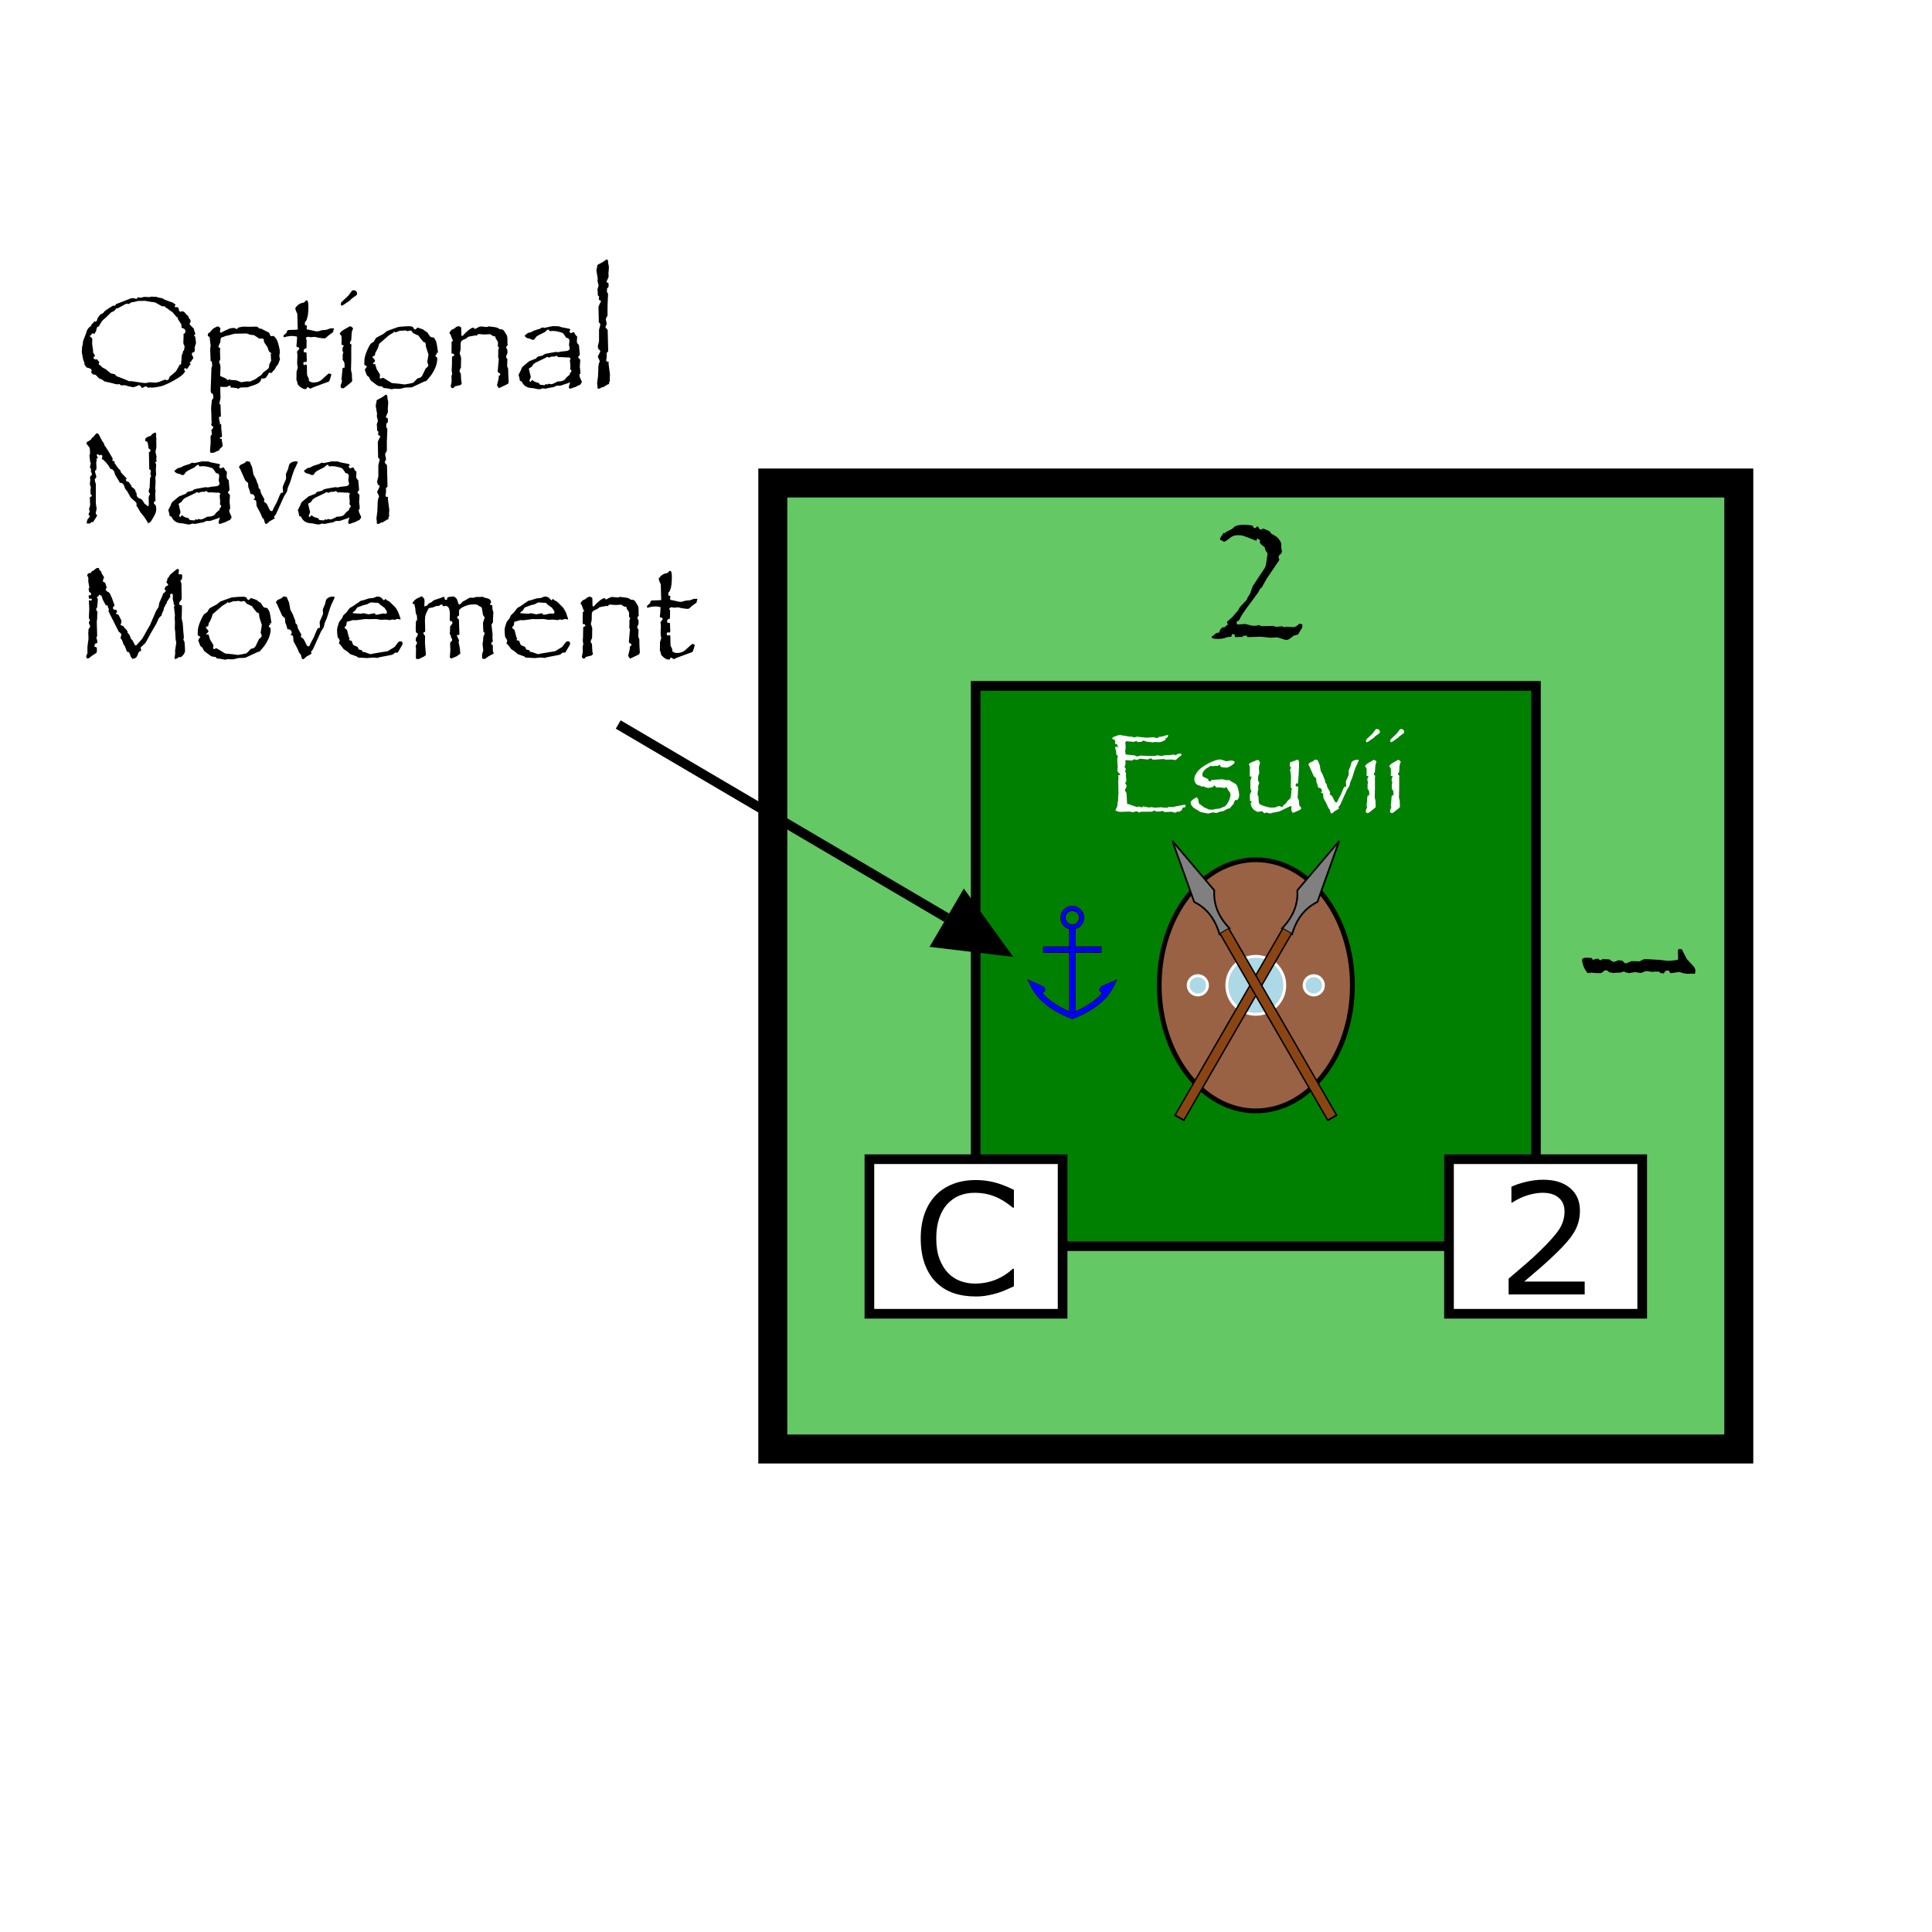
\includegraphics[width=0.75\linewidth]{Naval_Unit_Description.png}

\textit{Designer's Note: Historically only the coastal tribes built and used ships. Caesar only describes the Veneti ships in any detail.}